\documentclass[12pt,a4paper]{article}

% ─── Packages ────────────────────────────────────────────────────────────────
\usepackage[a4paper, top=2.5cm, bottom=2.5cm, left=2.8cm, right=2.8cm]{geometry}
\setlength{\emergencystretch}{4em}
\usepackage[table,xcdraw]{xcolor}
\usepackage{booktabs}
\usepackage{tabularx}
\usepackage{longtable}
\usepackage{multirow}
\usepackage{array}
\usepackage{fancyhdr}
\usepackage{titlesec}
\usepackage{hyperref}
\usepackage{enumitem}
\usepackage{tikz}
\usepackage{tcolorbox}
\usepackage{mdframed}
\usepackage{parskip}
\usepackage{graphicx}
\usepackage{amsmath}
\usepackage{microtype}
\usepackage{seqsplit}
\usepackage{mathptmx}
\usepackage[scaled=0.92]{helvet}
\usepackage[T1]{fontenc}
\usepackage[utf8]{inputenc}

\tcbuselibrary{skins, breakable}
\usetikzlibrary{shapes.geometric, arrows.meta, positioning, fit, backgrounds}
\setlength{\headheight}{15pt}

% ─── Colours ─────────────────────────────────────────────────────────────────
\definecolor{primary}{HTML}{C0392B}      % deep red
\definecolor{primarydark}{HTML}{922B21}  % darker red
\definecolor{secondary}{HTML}{2C3E50}    % dark navy
\definecolor{accent}{HTML}{E74C3C}       % bright red
\definecolor{lightgray}{HTML}{F5F6FA}
\definecolor{tabhead}{HTML}{2C3E50}
\definecolor{tabaltrow}{HTML}{FDFEFE}
\definecolor{success}{HTML}{1E8449}
\definecolor{successbg}{HTML}{D5F5E3}
\definecolor{infobg}{HTML}{D6EAF8}
\definecolor{warningbg}{HTML}{FDEBD0}
\definecolor{codebg}{HTML}{F2F3F4}

% ─── Hyperref setup ──────────────────────────────────────────────────────────
\hypersetup{
    colorlinks=true,
    linkcolor=primary,
    urlcolor=primary,
    citecolor=primary,
    pdftitle={Food Ordering System -- SRS},
    pdfauthor={Software Engineering Team},
    pdfsubject={Software Requirements Specification},
}

% ─── Header / Footer ─────────────────────────────────────────────────────────
\pagestyle{fancy}
\fancyhf{}
\fancyhead[L]{\small\textcolor{secondary}{\textbf{Food Ordering System}}}
\fancyhead[R]{\small\textcolor{secondary}{Software Requirements Specification}}
\fancyfoot[C]{\small\textcolor{gray}{\thepage}}
\fancyfoot[L]{\small\textcolor{gray}{Fundamentals of Software Engineering --- Phase 1}}
\renewcommand{\headrulewidth}{0.4pt}
\renewcommand{\footrulewidth}{0.4pt}
\renewcommand{\headrule}{\hbox to\headwidth{\color{primary}\leaders\hrule height \headrulewidth\hfill}}
\renewcommand{\footrule}{\hbox to\headwidth{\color{primary}\leaders\hrule height \footrulewidth\hfill}}

% ─── Section styling ─────────────────────────────────────────────────────────
\titleformat{\section}
  {\Large\bfseries\color{primary}}
  {\thesection}{1em}{}
  [\vspace{-0.3em}\textcolor{primary}{\rule{\linewidth}{0.6pt}}\vspace{0.2em}]

\titleformat{\subsection}
  {\large\bfseries\color{secondary}}
  {\thesubsection}{1em}{}

\titleformat{\subsubsection}
  {\normalsize\bfseries\color{secondary}}
  {\thesubsubsection}{1em}{}

% ─── Custom tcolorbox styles ─────────────────────────────────────────────────
\tcbset{
  infostyle/.style={
    enhanced, breakable,
    colback=infobg, colframe=secondary!60,
    fonttitle=\bfseries\small, coltitle=secondary,
    boxrule=0.4pt, arc=3pt,
    left=6pt, right=6pt, top=4pt, bottom=4pt,
  },
  reqstyle/.style={
    enhanced, breakable,
    colback=lightgray, colframe=primary!50,
    boxrule=0.4pt, arc=3pt,
    left=6pt, right=6pt, top=4pt, bottom=4pt,
  },
  notestyle/.style={
    enhanced,
    colback=warningbg, colframe=accent!70,
    fonttitle=\bfseries\small\color{primary},
    boxrule=0.4pt, arc=3pt,
    left=6pt, right=6pt, top=4pt, bottom=4pt,
  },
}

% ─── Table helpers ───────────────────────────────────────────────────────────
\newcommand{\thead}[1]{\textbf{\textcolor{white}{#1}}}
\newcolumntype{L}[1]{>{\raggedright\arraybackslash}p{#1}}
\newcolumntype{C}[1]{>{\centering\arraybackslash}p{#1}}

% row colours for tables
\rowcolors{2}{tabaltrow}{lightgray}

% ─── Misc helpers ────────────────────────────────────────────────────────────
\newcommand{\code}[1]{\texttt{\footnotesize\colorbox{codebg}{#1}}}
% \tcode: breakable code for table cells (no background box)
\newcommand{\tcode}[1]{{\footnotesize\ttfamily\seqsplit{#1}}}
\newcommand{\reqid}[1]{\textbf{\textcolor{primary}{#1}}}
\newcommand{\priority}[1]{%
  \ifstrequal{#1}{Must Have}{\textcolor{primary}{\textbf{Must Have}}}{%
  \ifstrequal{#1}{Should Have}{\textcolor{secondary}{\textbf{Should Have}}}{%
  \textcolor{gray}{#1}}}%
}

% ─────────────────────────────────────────────────────────────────────────────
\begin{document}
\sloppy
\tolerance=3000
\hbadness=3000
\pagenumbering{gobble}   % no page number on title page

% ═══════════════════════════════════════════════════════════════════════════
%  TITLE PAGE
% ═══════════════════════════════════════════════════════════════════════════
\begin{tikzpicture}[remember picture, overlay]
  % Top banner
  \fill[primary] (current page.north west) rectangle
    ([yshift=-4.5cm]current page.north east);
  % Bottom accent strip
  \fill[secondary] (current page.south west) rectangle
    ([yshift=1.2cm]current page.south east);
  \fill[accent] ([yshift=1.2cm]current page.south west) rectangle
    ([yshift=1.6cm]current page.south east);
\end{tikzpicture}

\vspace*{1.2cm}
\begin{center}
  {\fontsize{36}{42}\selectfont\bfseries\textcolor{white}{Food Ordering System}}\\[0.4cm]
  {\Large\textcolor{white!80!primary}{Software Requirements Specification}}\\[0.2cm]
  {\normalsize\textcolor{white!60!primary}{Version 1.0}}
\end{center}

\vspace{3.0cm}

\begin{center}
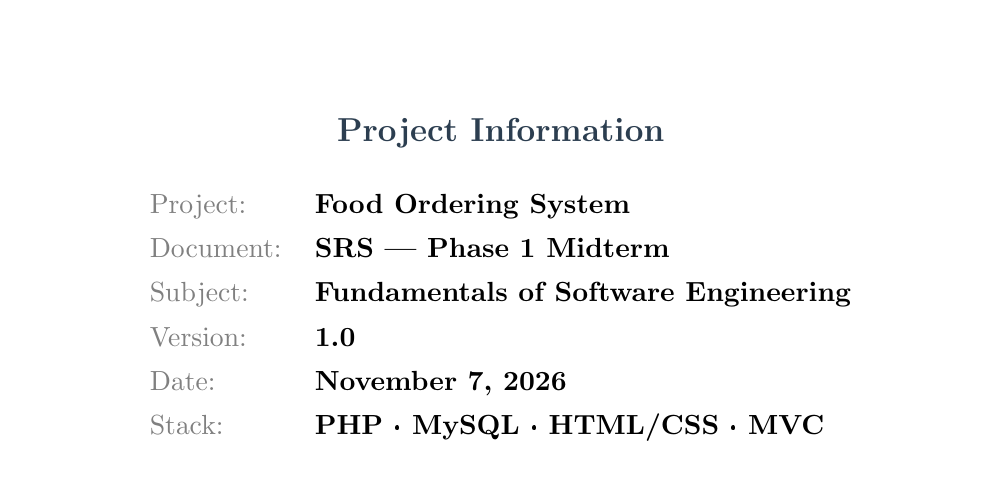
\begin{tikzpicture}
  \node[draw=white, fill=white, rounded corners=8pt, minimum width=12cm,
        minimum height=5.5cm] (box) {};
  \node[anchor=north] at (box.north) [yshift=-0.5cm] {%
    \begin{minipage}{11cm}
      \centering
      {\large\bfseries\textcolor{secondary}{Project Information}}\\[0.5cm]
      \begin{tabular}{@{}ll@{}}
        \textcolor{gray}{Project:}   & \textbf{Food Ordering System} \\[4pt]
        \textcolor{gray}{Document:}  & \textbf{SRS --- Phase 1 Midterm} \\[4pt]
        \textcolor{gray}{Subject:}   & \textbf{Fundamentals of Software Engineering} \\[4pt]
        \textcolor{gray}{Version:}   & \textbf{1.0} \\[4pt]
        \textcolor{gray}{Date:}      & \textbf{\today} \\[4pt]
        \textcolor{gray}{Stack:}     & \textbf{PHP · MySQL · HTML/CSS · MVC} \\[4pt]
      \end{tabular}
    \end{minipage}
  };
\end{tikzpicture}
\end{center}

\vfill
\begin{center}
  \textcolor{white}{\small Fundamentals of Software Engineering \quad|\quad Phase 1 Submission}
\end{center}
\vspace{0.6cm}

\newpage
\pagenumbering{roman}

% ═══════════════════════════════════════════════════════════════════════════
%  TABLE OF CONTENTS
% ═══════════════════════════════════════════════════════════════════════════
\tableofcontents
\newpage
\pagenumbering{arabic}

% ═══════════════════════════════════════════════════════════════════════════
%  1. INTRODUCTION
% ═══════════════════════════════════════════════════════════════════════════
\section{Introduction}

\subsection{Purpose}

This Software Requirements Specification (SRS) document describes the complete set of
functional and non-functional requirements for the \textbf{Food Ordering System} --- a
PHP-based web application developed as a Phase 1 midterm project for the Fundamentals
of Software Engineering course.

The system allows customers to browse food menus, place orders via an interactive cart,
and print invoices, while providing administrators with full CRUD control over all
seven database entities.

\subsection{Scope}

The Food Ordering System covers the following functional scope:

\begin{itemize}[leftmargin=1.5em, itemsep=3pt]
  \item Role-based authentication with \textbf{Admin} and \textbf{Customer} roles.
  \item Full CRUD management for \textbf{7 database tables}: \code{users},
        \code{user\_types}, \code{menu}, \code{products}, \code{orders},
        \code{order\_details}, and \code{usertype\_menu}.
  \item Customer-facing menu browsing with a live cart and one-click ordering.
  \item Printable, formatted invoices for every placed order.
  \item Admin dashboard with real-time statistics.
  \item Role-to-menu mapping management (\code{usertype\_menu}).
\end{itemize}

\subsection{Definitions and Acronyms}

\rowcolors{2}{lightgray}{tabaltrow}
\begin{tabularx}{\linewidth}{@{} L{2.8cm} X @{}}
  \rowcolor{tabhead}
  \thead{Term} & \thead{Definition} \\
  CRUD    & Create, Read, Update, Delete --- the four fundamental database operations \\
  MVC     & Model-View-Controller --- the architectural pattern used throughout the project \\
  PDO     & PHP Data Objects --- the database abstraction layer for all SQL queries \\
  SRS     & Software Requirements Specification --- this document \\
  Admin   & A privileged user who manages all system data \\
  Customer & A regular end-user who browses menus and places food orders \\
  Session & PHP server-side mechanism (\code{\$\_SESSION}) for maintaining login state \\
  FR      & Functional Requirement \\
  NFR     & Non-Functional Requirement \\
  bcrypt  & Password hashing algorithm used via PHP's \code{password\_hash()} \\
  LAMP    & Linux, Apache, MySQL, PHP --- the server stack the system targets \\
\end{tabularx}

\subsection{Document Overview}

\begin{itemize}[leftmargin=1.5em, itemsep=2pt]
  \item \textbf{Section 2} --- Overall system description, user classes, and constraints.
  \item \textbf{Section 3} --- Functional requirements (15 requirements).
  \item \textbf{Section 4} --- Non-functional requirements (6 requirements).
  \item \textbf{Section 5} --- Detailed class descriptions (17 classes).
  \item \textbf{Section 6} --- Use case descriptions (10 use cases).
  \item \textbf{Section 7} --- Database schema overview.
\end{itemize}

% ═══════════════════════════════════════════════════════════════════════════
%  2. OVERALL DESCRIPTION
% ═══════════════════════════════════════════════════════════════════════════
\section{Overall Description}

\subsection{Product Perspective}

The Food Ordering System is a \textbf{standalone web application} built in pure PHP using
a custom MVC architecture with no external framework dependency. It runs on any standard
LAMP/WAMP/XAMPP stack and uses MySQL as its relational database backend.

The system replaces a manual, paper-based ordering process with a digital, role-aware
interface that serves both kitchen staff (Admin) and walk-in or remote customers.

\subsection{Product Functions}

\begin{tcolorbox}[reqstyle]
\begin{itemize}[leftmargin=1.5em, itemsep=4pt]
  \item \textbf{Authentication} --- Login/logout with bcrypt-hashed passwords and PHP
        session management.
  \item \textbf{Admin Panel} --- Dashboard with summary statistics, and full CRUD for
        all 7 database tables via modal dialogs.
  \item \textbf{Customer Interface} --- Browse menu categories, add items to an interactive
        cart, and place orders in a single step.
  \item \textbf{Order Lifecycle} --- Status tracking through
        \textit{pending} $\rightarrow$ \textit{processing} $\rightarrow$ \textit{delivered}
        (or \textit{cancelled}).
  \item \textbf{Invoice Printing} --- Formatted, print-ready invoice for any order,
        accessible by both Admin and Customer.
\end{itemize}
\end{tcolorbox}

\subsection{User Classes and Characteristics}

\rowcolors{2}{lightgray}{tabaltrow}
\begin{tabularx}{\linewidth}{@{} L{2.5cm} L{4.5cm} X @{}}
  \rowcolor{tabhead}
  \thead{User Class} & \thead{Description} & \thead{Access} \\
  \textbf{Admin}
    & System administrator. Full control over all data and system configuration.
    & All pages: users, user types, menus, products, orders, order details,
      role-menu mapping, dashboards, invoices. \\
  \textbf{Customer}
    & Registered end-user who places food orders.
    & Browse menu, place orders, view personal order history, print own invoices. \\
\end{tabularx}

\subsection{Operating Environment}

\begin{itemize}[leftmargin=1.5em, itemsep=3pt]
  \item \textbf{Server:} Apache 2.4+ or Nginx with PHP 7.4 or higher.
  \item \textbf{Database:} MySQL 5.7+ or MariaDB 10.3+.
  \item \textbf{Client:} Any modern browser (Chrome, Firefox, Edge, Safari).
  \item \textbf{Development Stack:} XAMPP or WAMP (Windows), LAMP (Linux).
\end{itemize}

\subsection{Assumptions and Dependencies}

\begin{itemize}[leftmargin=1.5em, itemsep=3pt]
  \item The MySQL server is accessible at \code{localhost} with the credentials
        defined in \code{app/config/database.php}.
  \item The database \code{food\_ordering\_system} has been created and seeded
        by running \code{database.sql}.
  \item \code{public/setup.php} has been executed once to set correct bcrypt
        password hashes for demo accounts.
  \item No Composer or third-party PHP libraries are required.
\end{itemize}

% ═══════════════════════════════════════════════════════════════════════════
%  3. FUNCTIONAL REQUIREMENTS
% ═══════════════════════════════════════════════════════════════════════════
\section{Functional Requirements}

Each requirement is identified by a unique ID, with a priority classification of
\textbf{Must Have} (critical) or \textbf{Should Have} (important but not blocking).

\vspace{0.5em}

% --- FR-01 through FR-07 ---
{\setlength{\tabcolsep}{3pt}
\setlength{\LTleft}{0pt}\setlength{\LTright}{0pt}
\begin{longtable}{ p{1.0cm} p{2.3cm} p{5.0cm} p{1.7cm} p{3.8cm} }
  \rowcolor{tabhead}
  \thead{ID} & \thead{Name} & \thead{Description} & \thead{Priority} & \thead{Impl.\ Reference} \\
  \endfirsthead
  \rowcolor{tabhead}
  \thead{ID} & \thead{Name} & \thead{Description} & \thead{Priority} & \thead{Impl.\ Reference} \\
  \endhead

  \rowcolor{tabaltrow}
  \reqid{FR-01} & User Authentication
    & The system shall allow users to log in using their email address and password.
      Invalid credentials redirect back to login with an error message.
    & Must Have
    & \tcode{LoginController::login()} with \tcode{password\_verify()} \\

  \rowcolor{lightgray}
  \reqid{FR-02} & Role-Based Dashboards
    & The system shall redirect authenticated users to role-specific dashboards:
      Admin to the admin panel, Customer to the customer home.
    & Must Have
    & \tcode{public/index.php} router; admin and customer dashboard views \\

  \rowcolor{tabaltrow}
  \reqid{FR-03} & User Management (CRUD)
    & Admin shall create, read, update, and delete user accounts. Each user
      is assigned a role from the \tcode{user\_types} table.
    & Must Have
    & \tcode{UserController}, \tcode{User} model, \tcode{users/index.php} \\

  \rowcolor{lightgray}
  \reqid{FR-04} & User Type Management (CRUD)
    & Admin shall manage user roles with full CRUD on the \tcode{user\_types} table.
    & Must Have
    & \tcode{UserTypeController}, \tcode{UserType} model \\

  \rowcolor{tabaltrow}
  \reqid{FR-05} & Menu Management (CRUD)
    & Admin shall create, read, update, and delete menu categories. Each menu
      has a name and description.
    & Must Have
    & \tcode{MenuController}, \tcode{Menu} model \\

  \rowcolor{lightgray}
  \reqid{FR-06} & Product Management (CRUD)
    & Admin shall add, edit, and delete products. Each product has a name,
      price, and belongs to a menu category.
    & Must Have
    & \tcode{ProductController}, \tcode{Product} model \\

  \rowcolor{tabaltrow}
  \reqid{FR-07} & Order Management (CRUD)
    & Admin shall view all orders across all users, update order status, and
      delete orders. Orders display the customer name via a JOIN.
    & Must Have
    & \tcode{OrderController}, \tcode{Order} model \\

  \rowcolor{lightgray}
  \reqid{FR-08} & Order Detail Management (CRUD)
    & Admin shall manage individual line items within orders: product,
      quantity, and computed price. Price auto-calculates on product selection.
    & Must Have
    & \tcode{OrderDetailController}, \tcode{OrderDetail} model \\

  \rowcolor{tabaltrow}
  \reqid{FR-09} & Role-Menu Mapping (CRUD)
    & Admin shall assign which menu categories are visible to which user types
      via the \tcode{usertype\_menu} join table.
    & Should Have
    & \tcode{UserTypeMenuController}, \tcode{UserTypeMenu} model \\

  \rowcolor{lightgray}
  \reqid{FR-10} & Browse Menu
    & Customers shall browse all available products grouped by menu category,
      with item names and prices displayed on cards.
    & Must Have
    & \tcode{customer/browse\_menu.php} with product grouping logic \\

  \rowcolor{tabaltrow}
  \reqid{FR-11} & Interactive Cart
    & Customers shall increment/decrement item quantities; the cart updates
      totals in real time without a page reload using JavaScript.
    & Must Have
    & JavaScript cart in \tcode{browse\_menu.php}; cart modal \\

  \rowcolor{lightgray}
  \reqid{FR-12} & Place Order
    & Customers shall submit their cart to create an order record and
      corresponding order detail records in a single transaction.
    & Must Have
    & \tcode{CustomerDashboardController} \tcode{::placeOrder()}; \tcode{Order::create()} returns \tcode{lastInsertId} \\

  \rowcolor{tabaltrow}
  \reqid{FR-13} & My Orders
    & Customers shall view a history of all their own orders, filtered by
      their \tcode{user\_id}, with status badges.
    & Must Have
    & \tcode{customer/my\_orders.php}; array\_filter on \tcode{user\_id} \\

  \rowcolor{lightgray}
  \reqid{FR-14} & Print Invoice
    & Any user shall print a formatted invoice for any of their orders.
      Admin can print invoices for all orders. The print layout hides
      navigation and action buttons.
    & Must Have
    & \tcode{app/views/invoice.php}; \tcode{@media print} CSS \\

  \rowcolor{tabaltrow}
  \reqid{FR-15} & Logout
    & The system shall destroy the PHP session and redirect the user to the
      login page when the logout link is clicked.
    & Must Have
    & \tcode{LoginController::logout()}; \tcode{session\_destroy()} \\

\end{longtable}
}

\newpage
% ═══════════════════════════════════════════════════════════════════════════
%  4. NON-FUNCTIONAL REQUIREMENTS
% ═══════════════════════════════════════════════════════════════════════════
\section{Non-Functional Requirements}

\begin{tabular*}{\linewidth}{@{\extracolsep{\fill}} p{1.0cm} p{3.2cm} p{5.0cm} p{4.0cm} @{}}
  \rowcolor{tabhead}
  \thead{ID} & \thead{Category} & \thead{Description} & \thead{Code Reference} \\

  \reqid{NFR-01} & Security
    & All user passwords are stored using the bcrypt algorithm via PHP's
      \tcode{PASSWORD\_DEFAULT} constant (cost factor 10). PDO prepared
      statements with named placeholders are used for every database query,
      preventing SQL injection. Session-based access control blocks
      unauthenticated access to all protected routes.
    & \tcode{User::create()} calls \tcode{password\_hash()};
      \tcode{User::findByEmail()} calls \tcode{password\_verify()};
      all models use \tcode{PDO::prepare()} \\

  \reqid{NFR-02} & Maintainability
    & The system follows the MVC architectural pattern: models handle data
      access, controllers handle HTTP logic, and views handle presentation.
      The \tcode{CrudInterface} enforces a uniform four-method contract across
      all seven models.
    & \tcode{CrudInterface.php} on all 7 models;
      one controller per entity \\

  \reqid{NFR-03} & Usability
    & The interface uses a responsive CSS grid layout with no external CSS
      frameworks. CRUD operations open in modal dialogs, avoiding full-page
      reloads. Order statuses are colour-coded with badges (green = delivered,
      amber = pending, red = cancelled) for fast visual scanning.
    & \tcode{assets/css/style.css}; modal-overlay pattern in all CRUD views;
      JavaScript \tcode{openModal()} / \tcode{closeModal()} helpers \\

  \reqid{NFR-04} & Reliability
    & All database operations use PDO with \tcode{ERRMODE\_EXCEPTION}, so
      failures surface as exceptions rather than silent failures. The
      \tcode{Order::create()} method returns the new row's ID directly via
      \tcode{lastInsertId()} on the same connection, preventing race conditions.
    & \tcode{Database::connect()} sets \tcode{PDO::ATTR\_ERRMODE};
      \tcode{Order::create()} returns \tcode{\$this->conn->lastInsertId()} \\

  \reqid{NFR-05} & Portability
    & The system has zero Composer or npm runtime dependencies. It runs on
      any LAMP, WAMP, or XAMPP stack with PHP $\geq$ 7.4 and MySQL 5.7+.
      No \tcode{.htaccess} rewrite rules are required; the front controller
      is accessed directly via \tcode{public/index.php}.
    & No \tcode{composer.json}; pure PHP, no framework \\

  \reqid{NFR-06} & Printability
    & The invoice page includes \tcode{@media print} CSS rules that hide the
      navigation bar, buttons, and all chrome, producing a clean, professional
      paper-ready layout suitable for handing to a customer.
    & \tcode{invoice.php}; \tcode{@media print} in \tcode{style.css} \\


\end{tabular*}

% ═══════════════════════════════════════════════════════════════════════════
%  5. CLASS DESCRIPTIONS
% ═══════════════════════════════════════════════════════════════════════════
\section{Detailed Class Descriptions}

The system is composed of \textbf{17 classes} across four layers: configuration,
interface, models, and controllers. All model classes implement \code{CrudInterface}.

\begin{tcolorbox}[infostyle, title=Architecture Note]
  \textbf{Interface Realization:} \code{CrudInterface} declares
  \code{create(\$data)}, \code{read()}, \code{update(\$id, \$data)}, and
  \code{delete(\$id)}. Every model class implements this interface, ensuring
  a uniform CRUD contract enforced at compile time by PHP.
\end{tcolorbox}

\vspace{0.5em}

\subsubsection*{Configuration \& Interface Layer}

\rowcolors{2}{lightgray}{tabaltrow}
\begin{tabularx}{\linewidth}{@{} L{2.8cm} L{3.2cm} L{3.2cm} X @{}}
  \rowcolor{tabhead}
  \thead{Class} & \thead{File} & \thead{Methods} & \thead{Responsibility} \\
  \tcode{Database}
    & \tcode{config/database.php}
    & \tcode{connect()}
    & Creates and returns a PDO connection. Sets error mode to
      \tcode{ERRMODE\_EXCEPTION}. Host, DB name, username, and password
      are private attributes. \\
  \tcode{CrudInterface}
    & \tcode{interfaces/} \tcode{CrudInterface.php}
    & \tcode{create}, \tcode{read}, \tcode{update}, \tcode{delete}
    & PHP interface defining the four-method CRUD contract enforced
      on all seven model classes. \\
\end{tabularx}

\vspace{0.8em}
\subsubsection*{Model Layer (7 Models --- all implement CrudInterface)}

\rowcolors{2}{lightgray}{tabaltrow}
\begin{tabularx}{\linewidth}{@{} L{2.8cm} L{3.2cm} L{3.2cm} X @{}}
  \rowcolor{tabhead}
  \thead{Class} & \thead{File} & \thead{Extra Methods} & \thead{Responsibility} \\
  \tcode{User}
    & \tcode{models/User.php}
    & \tcode{findByEmail(\$e)}
    & Manages \tcode{users} table. \tcode{create()} hashes the password with
      \tcode{password\_hash()}. \tcode{read()} JOINs \tcode{user\_types}
      to include role name. \\
  \tcode{UserType}
    & \tcode{models/UserType.php}
    & ---
    & Manages \tcode{user\_types} table. Stores role names such as
      \textit{Admin} and \textit{Customer}. \\
  \tcode{Menu}
    & \tcode{models/Menu.php}
    & ---
    & Manages \tcode{menu} table (food categories). Stores name and
      description. \\
  \tcode{Product}
    & \tcode{models/product.php}
    & ---
    & Manages \tcode{products} table. Each product has a name, price,
      and foreign key to \tcode{menu}. \tcode{read()} JOINs \tcode{menu}. \\
  \tcode{Order}
    & \tcode{models/Order.php}
    & ---
    & Manages \tcode{orders} table. \tcode{create()} returns
      \tcode{lastInsertId()} for use by \tcode{OrderDetail}. \tcode{read()}
      JOINs \tcode{users} for the customer name. \\
  \tcode{OrderDetail}
    & \tcode{models/orderDetail.php}
    & ---
    & Manages \tcode{order\_details} line items. Stores order ID, product
      ID, quantity, and computed price. \tcode{read()} JOINs
      \tcode{products}. \\
  \tcode{UserTypeMenu}
    & \tcode{models/UserTypeMenu.php}
    & ---
    & Manages \tcode{usertype\_menu} join table. Maps user type IDs to
      menu IDs. \tcode{read()} JOINs both \tcode{user\_types} and
      \tcode{menu}. \\
\end{tabularx}

\vspace{0.8em}
\subsubsection*{Controller Layer (8 Controllers)}

\rowcolors{2}{lightgray}{tabaltrow}
\begin{tabularx}{\linewidth}{@{} L{3.2cm} L{4cm} X @{}}
  \rowcolor{tabhead}
  \thead{Class} & \thead{Methods} & \thead{Responsibility} \\
  \tcode{LoginController}
    & \tcode{showLogin()}, \tcode{login()}, \tcode{logout()}
    & Renders login form; verifies credentials with \tcode{password\_verify()};
      sets \tcode{\$\_SESSION} on success; calls \tcode{session\_destroy()} on
      logout. \\
  \tcode{UserController}
    & \tcode{index()}, \tcode{store()}, \tcode{update()}, \tcode{delete()}
    & Full HTTP CRUD handler for users. Passes user types to the view for the
      role dropdown. \\
  \tcode{UserTypeController}
    & \tcode{index()}, \tcode{store()}, \tcode{update()}, \tcode{delete()}
    & Full HTTP CRUD handler for user types (roles). \\
  \tcode{MenuController}
    & \tcode{index()}, \tcode{store()}, \tcode{update()}, \tcode{delete()}
    & Full HTTP CRUD handler for menu categories. \\
  \tcode{ProductController}
    & \tcode{index()}, \tcode{store()}, \tcode{update()}, \tcode{delete()}
    & Full HTTP CRUD handler for products. Passes menu list for the category
      dropdown. \\
  \tcode{OrderController}
    & \tcode{index()}, \tcode{store()}, \tcode{update()}, \tcode{delete()}
    & Full HTTP CRUD handler for orders. Passes user list for the customer
      dropdown. \\
  \tcode{OrderDetailController}
    & \tcode{index()}, \tcode{store()}, \tcode{update()}, \tcode{delete()}
    & Full HTTP CRUD handler for order line items. Passes orders and products
      for dropdowns; price auto-computed client-side. \\
  \tcode{UserTypeMenuController}
    & \tcode{index()}, \tcode{store()}, \tcode{update()}, \tcode{delete()}
    & Full HTTP CRUD handler for role-menu mappings. \\
\end{tabularx}

% ═══════════════════════════════════════════════════════════════════════════
%  6. USE CASES
% ═══════════════════════════════════════════════════════════════════════════
\section{Use Case Descriptions}

\begin{tcolorbox}[infostyle, title=Actors]
  \textbf{Admin} --- System administrator with full access. \quad
  \textbf{Customer} --- Registered user with order access.
\end{tcolorbox}

\vspace{0.5em}

% UC-01
\begin{mdframed}[linecolor=primary!40, linewidth=0.6pt, roundcorner=4pt,
                 backgroundcolor=lightgray, innerleftmargin=10pt, innerrightmargin=10pt,
                 innertopmargin=8pt, innerbottommargin=8pt]
\textbf{\textcolor{primary}{UC-01} \quad Login}

\vspace{3pt}
\begin{tabular}{@{} L{2.6cm} p{11.6cm} @{}}
  \textit{Actor(s)}   & Admin, Customer \\
  \textit{Trigger}    & User navigates to \tcode{index.php?action=login} \\
  \textit{Main Flow}  & 1. System displays login form. \newline
                        2. User enters email and password and submits. \newline
                        3. \tcode{LoginController::login()} fetches user by email. \newline
                        4. \tcode{password\_verify()} checks the bcrypt hash. \newline
                        5. On success: session variables set; Admin $\to$ admin dashboard, Customer $\to$ customer dashboard. \\
  \textit{Alt. Flow}  & If credentials are invalid, redirect to login with \tcode{error=1} query param. \\
  \textit{Outcome}    & Authenticated PHP session created; user on their role dashboard. \\
\end{tabular}
\end{mdframed}

\vspace{0.6em}

% UC-02
\begin{mdframed}[linecolor=primary!40, linewidth=0.6pt, roundcorner=4pt,
                 backgroundcolor=lightgray, innerleftmargin=10pt, innerrightmargin=10pt,
                 innertopmargin=8pt, innerbottommargin=8pt]
\textbf{\textcolor{primary}{UC-02} \quad Manage Users (Admin CRUD)}

\vspace{3pt}
\begin{tabular}{@{} L{2.6cm} p{11.6cm} @{}}
  \textit{Actor(s)}  & Admin \\
  \textit{Trigger}   & Admin clicks \textbf{Users} in the navigation bar \\
  \textit{Main Flow} & 1. \tcode{UserController::index()} fetches all users (with role names). \newline
                       2. Admin sees a table of users with Edit / Delete buttons. \newline
                       3. \textbf{Create:} Click ``+ Add User'' $\to$ modal form $\to$ POST to \tcode{user\_create}. \newline
                       4. \textbf{Update:} Click ``Edit'' $\to$ modal pre-filled $\to$ POST to \tcode{user\_update}. \newline
                       5. \textbf{Delete:} Click ``Delete'' $\to$ confirm dialog $\to$ GET \tcode{user\_delete\&id=N}. \\
  \textit{Outcome}   & User record created, updated, or removed in \tcode{users} table. \\
\end{tabular}
\end{mdframed}

\vspace{0.6em}

% UC-03
\begin{mdframed}[linecolor=primary!40, linewidth=0.6pt, roundcorner=4pt,
                 backgroundcolor=lightgray, innerleftmargin=10pt, innerrightmargin=10pt,
                 innertopmargin=8pt, innerbottommargin=8pt]
\textbf{\textcolor{primary}{UC-03} \quad Manage Menus, Products, User Types, Role-Menu Mapping}

\vspace{3pt}
\begin{tabular}{@{} L{2.6cm} p{11.6cm} @{}}
  \textit{Actor(s)}  & Admin \\
  \textit{Trigger}   & Admin clicks the relevant item in the navigation bar \\
  \textit{Main Flow} & 1. Controller fetches the relevant records. \newline
                       2. Admin views the table with inline Edit / Delete actions. \newline
                       3. Create / Update / Delete follow the same modal pattern as UC-02. \\
  \textit{Scope}     & Applies to: \tcode{menu}, \tcode{products}, \tcode{user\_types}, \tcode{usertype\_menu} \\
  \textit{Outcome}   & Record persisted, updated, or deleted in the respective table. \\
\end{tabular}
\end{mdframed}

\vspace{0.6em}

% UC-04
\begin{mdframed}[linecolor=primary!40, linewidth=0.6pt, roundcorner=4pt,
                 backgroundcolor=lightgray, innerleftmargin=10pt, innerrightmargin=10pt,
                 innertopmargin=8pt, innerbottommargin=8pt]
\textbf{\textcolor{primary}{UC-04} \quad Manage Orders \& Order Details}

\vspace{3pt}
\begin{tabular}{@{} L{2.6cm} p{11.6cm} @{}}
  \textit{Actor(s)}  & Admin \\
  \textit{Trigger}   & Admin clicks \textbf{Orders} or \textbf{Order Details} \\
  \textit{Main Flow} & 1. Controller fetches records (with JOINs for customer/product names). \newline
                       2. Admin can update order status (pending / processing / delivered / cancelled). \newline
                       3. Admin can delete an order or individual line item. \newline
                       4. Admin can click \textbf{Invoice} to open the printable invoice in a new tab. \\
  \textit{Outcome}   & Order status updated; line items managed; invoice accessible. \\
\end{tabular}
\end{mdframed}

\vspace{0.6em}

% UC-05
\begin{mdframed}[linecolor=primary!40, linewidth=0.6pt, roundcorner=4pt,
                 backgroundcolor=lightgray, innerleftmargin=10pt, innerrightmargin=10pt,
                 innertopmargin=8pt, innerbottommargin=8pt]
\textbf{\textcolor{primary}{UC-05} \quad Browse Menu \& Add to Cart}

\vspace{3pt}
\begin{tabular}{@{} L{2.6cm} p{11.6cm} @{}}
  \textit{Actor(s)}  & Customer \\
  \textit{Trigger}   & Customer clicks \textbf{Browse Menu} \\
  \textit{Main Flow} & 1. Products are fetched and grouped by menu category. \newline
                       2. Each product card shows name, price, and a quantity spinner. \newline
                       3. Customer adjusts quantities; cart total updates in real-time (JavaScript). \newline
                       4. Customer clicks \textbf{View Cart} to review items before ordering. \\
  \textit{Outcome}   & Cart populated in browser memory, ready to be submitted as an order. \\
\end{tabular}
\end{mdframed}

\vspace{0.6em}

% UC-06
\begin{mdframed}[linecolor=primary!40, linewidth=0.6pt, roundcorner=4pt,
                 backgroundcolor=lightgray, innerleftmargin=10pt, innerrightmargin=10pt,
                 innertopmargin=8pt, innerbottommargin=8pt]
\textbf{\textcolor{primary}{UC-06} \quad Place Order}

\vspace{3pt}
\begin{tabular}{@{} L{2.6cm} p{11.6cm} @{}}
  \textit{Actor(s)}  & Customer \\
  \textit{Trigger}   & Customer clicks \textbf{Place Order} in the cart modal \\
  \textit{Main Flow} & 1. Cart is POSTed to \tcode{index.php?action=place\_order}. \newline
                       2. Server computes total from product prices $\times$ quantities. \newline
                       3. \tcode{Order::create()} inserts a row into \tcode{orders} and returns \tcode{lastInsertId()}. \newline
                       4. \tcode{OrderDetail::create()} inserts one row per cart item into \tcode{order\_details}. \newline
                       5. Redirect to My Orders with a success message. \\
  \textit{Outcome}   & New order with status \textit{pending} created; order details persisted. \\
\end{tabular}
\end{mdframed}

\vspace{0.6em}

% UC-07
\begin{mdframed}[linecolor=primary!40, linewidth=0.6pt, roundcorner=4pt,
                 backgroundcolor=lightgray, innerleftmargin=10pt, innerrightmargin=10pt,
                 innertopmargin=8pt, innerbottommargin=8pt]
\textbf{\textcolor{primary}{UC-07} \quad View My Orders}

\vspace{3pt}
\begin{tabular}{@{} L{2.6cm} p{11.6cm} @{}}
  \textit{Actor(s)}  & Customer \\
  \textit{Trigger}   & Customer clicks \textbf{My Orders} in the navigation bar \\
  \textit{Main Flow} & 1. All orders are fetched; filtered client-side by the session \tcode{user\_id}. \newline
                       2. Orders are displayed newest-first with colour-coded status badges. \newline
                       3. Each row has a \textbf{Print Invoice} link. \\
  \textit{Outcome}   & Customer views their complete order history. \\
\end{tabular}
\end{mdframed}

\vspace{0.6em}

% UC-08
\begin{mdframed}[linecolor=primary!40, linewidth=0.6pt, roundcorner=4pt,
                 backgroundcolor=lightgray, innerleftmargin=10pt, innerrightmargin=10pt,
                 innertopmargin=8pt, innerbottommargin=8pt]
\textbf{\textcolor{primary}{UC-08} \quad Print Invoice}

\vspace{3pt}
\begin{tabular}{@{} L{2.6cm} p{11.6cm} @{}}
  \textit{Actor(s)}  & Admin, Customer \\
  \textit{Trigger}   & User clicks \textbf{Invoice} button for an order \\
  \textit{Main Flow} & 1. \tcode{CustomerDashboardController::printInvoice()} verifies that the
                           requesting user owns the order (or is Admin). \newline
                       2. Order details are fetched and rendered in \tcode{app/views/invoice.php}. \newline
                       3. Invoice opens in a new tab. \newline
                       4. User clicks \textbf{Print Invoice} to trigger the browser print dialog. \\
  \textit{Outcome}   & Formatted paper invoice printed. Navigation hidden by \tcode{@media print} CSS. \\
\end{tabular}
\end{mdframed}

\vspace{0.6em}

% UC-09
\begin{mdframed}[linecolor=primary!40, linewidth=0.6pt, roundcorner=4pt,
                 backgroundcolor=lightgray, innerleftmargin=10pt, innerrightmargin=10pt,
                 innertopmargin=8pt, innerbottommargin=8pt]
\textbf{\textcolor{primary}{UC-09} \quad Logout}

\vspace{3pt}
\begin{tabular}{@{} L{2.6cm} p{11.6cm} @{}}
  \textit{Actor(s)}  & Admin, Customer \\
  \textit{Trigger}   & User clicks \textbf{Logout} in the navigation bar \\
  \textit{Main Flow} & 1. Request routed to \tcode{LoginController::logout()}. \newline
                       2. \tcode{session\_destroy()} terminates the session. \newline
                       3. User redirected to the login page. \\
  \textit{Outcome}   & Session destroyed; user must log in again to access the system. \\
\end{tabular}
\end{mdframed}

% ═══════════════════════════════════════════════════════════════════════════
%  7. DATABASE SCHEMA
% ═══════════════════════════════════════════════════════════════════════════
\section{Database Schema}

The system uses \textbf{7 MySQL tables} with foreign-key relationships enforced
at the database level.

\rowcolors{2}{lightgray}{tabaltrow}
\begin{tabularx}{\linewidth}{@{} C{0.5cm} L{3.2cm} L{5cm} X @{}}
  \rowcolor{tabhead}
  \thead{\#} & \thead{Table} & \thead{Key Columns} & \thead{Description} \\
  1 & \tcode{user\_types}
    & \tcode{id}, \tcode{type\_name}
    & Roles: Admin, Customer. Referenced by \tcode{users}. \\
  2 & \tcode{users}
    & \tcode{id}, \tcode{name}, \tcode{email}, \tcode{password}, \tcode{user\_type\_id}
    & System accounts. Password stored as bcrypt hash. FK to \tcode{user\_types}. \\
  3 & \tcode{menu}
    & \tcode{id}, \tcode{name}, \tcode{description}
    & Food categories (Breakfast, Main Course, Desserts, Beverages). \\
  4 & \tcode{products}
    & \tcode{id}, \tcode{name}, \tcode{price}, \tcode{menu\_id}
    & Individual food items. FK to \tcode{menu}. \\
  5 & \tcode{orders}
    & \tcode{id}, \tcode{user\_id}, \tcode{total\_price}, \tcode{status}, \tcode{created\_at}
    & Customer orders. Status ENUM: pending / processing / delivered / cancelled.
      FK to \tcode{users}. \\
  6 & \tcode{order\_details}
    & \tcode{id}, \tcode{order\_id}, \tcode{product\_id}, \tcode{quantity}, \tcode{price}
    & Line items per order. FK to both \tcode{orders} and \tcode{products}. \\
  7 & \tcode{usertype\_menu}
    & \tcode{id}, \tcode{user\_type\_id}, \tcode{menu\_id}
    & Maps roles to accessible menus. Unique constraint on
      \tcode{(user\_type\_id, menu\_id)}. FK to \tcode{user\_types} and \tcode{menu}. \\
\end{tabularx}

\vspace{1em}

\begin{tcolorbox}[notestyle, title=Entity Relationship Summary]
\tcode{user\_types} $\xleftarrow{1}$\;\tcode{users}\;$\xrightarrow{N}$\;\tcode{orders}\;$\xrightarrow{N}$\;\tcode{order\_details}\;$\xrightarrow{N}$\;\tcode{products}\;$\xrightarrow{N}$\;\tcode{menu}

\vspace{4pt}
\tcode{user\_types} $\xleftarrow{N}$ \tcode{usertype\_menu} $\xrightarrow{N}$ \tcode{menu}
\end{tcolorbox}

% ═══════════════════════════════════════════════════════════════════════════
%  BACK COVER
% ═══════════════════════════════════════════════════════════════════════════
\newpage
\begin{tikzpicture}[remember picture, overlay]
  \fill[secondary] (current page.south west) rectangle (current page.north east);
  \fill[primary]   ([yshift=-6cm]current page.north west) rectangle
                   ([yshift=-6.5cm]current page.north east);
\end{tikzpicture}

\vspace*{2cm}
\begin{center}
  {\Huge\bfseries\textcolor{white}{Food Ordering System}}\\[0.6cm]
  {\Large\textcolor{white!70!secondary}{Software Requirements Specification}}\\[2cm]

  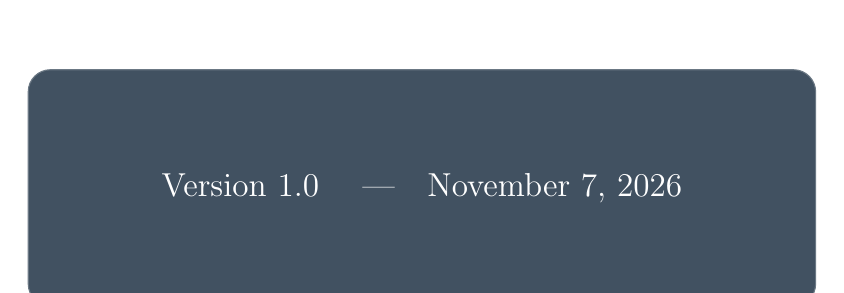
\begin{tikzpicture}
    \node[draw=white!30!secondary, fill=white!10!secondary, rounded corners=8pt,
          minimum width=10cm, minimum height=3cm] (box) {};
    \node at (box.center) {%
      \textcolor{white}{\large Version 1.0 \quad|\quad \today}
    };
  \end{tikzpicture}

  \vspace{2cm}
  {\normalsize\textcolor{white!60!secondary}{%
    Prepared for: Fundamentals of Software Engineering --- Phase 1}}
\end{center}

\end{document}
